\documentclass[12pt,a5paper]{article}

\usepackage[T1]{fontenc} % font encoding, lubab õ tähte kasutada
\usepackage[utf8]{inputenc} % oleme siiski 21. sajandis, vajadusel on ka olemas utf8x
\usepackage{lmodern} % lmodern ja micrtype käivad käsikäes, teeb teksti ilusamaks
\usepackage{microtype}
\usepackage[estonian]{babel} % eesti keele poolitamisreeglid jpm
\usepackage[per = fraction, expproduct=cdot, decimalsymbol=comma]{siunitx} % http://www.bakoma-tex.com/doc/latex/siunitx/siunitx.pdf
\usepackage{graphicx} 
\usepackage{wrapfig}
\usepackage{epstopdf} %minul on vaja, et .eps pilte saada
\usepackage{circuitikz}
\usepackage{tikz}
\usepackage{xcolor}
\usepackage{enumitem}
%paneme kõik mõõdud paika
\topmargin=-2.9cm \textheight=18.8cm \textwidth=12.77cm
\oddsidemargin=-1.5cm  \evensidemargin=-1.5cm
\setlength{\parindent}{0pt} \setlength{\parskip}{4pt} \sloppy
\relpenalty=10000 \binoppenalty=10000 % Tekstisisestes valemites reavahetusi ärgu olgu
\pagestyle{empty} % ilma leheküljenumbrita
\newcommand{\numb}[1]{\vspace{5pt}\textbf{\large #1}}
\newcommand{\nimi}[1]{(\textsl{\small #1})}
\newcommand{\punktid}[1]{(\emph{#1~p.})}
\newcounter{ylesanne}
\newcommand{\yl}[1]{\addtocounter{ylesanne}{1}\numb{\theylesanne.} \nimi{#1} \newblock{}}
\newcommand{\autor}[1]{\emph{ Autor: #1}}

\begin{document}

\begin{center}
\textbf{\Large Eesti koolinoorte 65. füüsikaolümpiaad} \vspace{2pt}

\emph{19. jaanuar 2019. a. Piirkondlik voor.}

\emph{Gümnaasiumi ülesanded (10. - 12. klass)}

\end{center}

\yl{RONG} Juku tahtis teada, mitu vagunit on rongis. Selleks seisis ta perroonile esimese vaguni esiotsaga kohakuti ning ootas, kuni rong ühtlase kiirendusega sõitmist alustas.
Stopperiga mõõtes sai ta teada, et esimene vagun läks temast mööda täpselt aja $t=\SI{10}{s}$ jooksul ning viimane vagun aja  $t_2 = \SI{1.83}{s}$ jooksul. Mitu vagunit oli rongis?
Vagunid on identsed. \punktid{6}

\begin{wrapfigure}[5]{r}{0.4\textwidth}
\vspace{-10pt}
	\begin{center}
		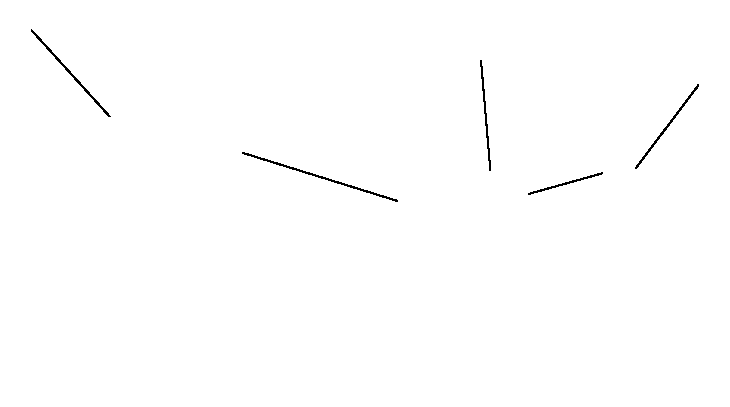
\includegraphics[width = 0.4\textwidth]{peegel}
	\end{center}
\end{wrapfigure}

\yl{PEEGEL} Optilises skeemis (vt. joonis) on kujutatud kolme valguskiire viit fragmenti. Samuti on teada, et skeemis on tasapeegel, mis on joonise tasandiga risti. Rekonstrueerige peegli asukoht. Ülesanne lahendage lisalehel. \punktid{6}


\yl{KÄRBES}
Kärbes asub kumerläätsest kümnekordse fookuskauguse kaugusel ning läätse optilisest peateljest kolme fookuskauguse kaugusel ning hakkab liikuma otse oma kujutise poole. Kui kaugel läätse tasandist asub kärbes hetkel, kui tema tõeline kujutis liigub kärbse suhtes\\
\osa kõige aeglasemalt;\\
\osa kõige kiiremini? Kui suur on kärbse kujutise kiirus kärbse suhtes nendel hetkedel? Põhjendage vastust. \punktid{8}

\yl{VAAKUM} Mõlemast otsast õhukindlalt suletud klaastoru pikkus $\ell=\SI{1}{m}$ ja sisediameeter $d=\SI{1}{cm}$. Õhurõhk $p=\SI{101.3}{kPa}$.\punktid{8}\\
\osa Kui palju tööd tuleb minimaalselt teha vaakumi tekitamiseks selles torus?\\
\osa Horisontaalse vakumeeritud toru ühes otsas on teraskuulike, mis saab l	ibiseda toru sees praktiliselt ilma hõõrdumiseta ja mille diameeter on võrdne toru sisediameetriga. Õnnetuse tõttu puruneb toru ots, mille lähedal kuulike paikneb  ja õhu surve paneb kuulikese liikuma vakumeeritud osa suunas. Kui suure kiiruse saavutab kuulike jõudes toru teise otsa? Terase tihedus on $\SI{7.9}{g/cm^3}$.





\begin{wrapfigure}[7]{r}{0.4\textwidth}
	\vspace{-15pt}
	\begin{center}
		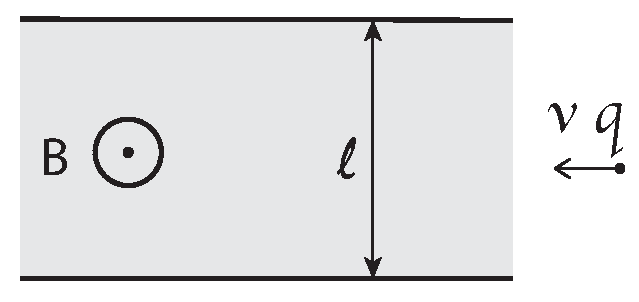
\includegraphics[width = 0.4\textwidth]{osakejoonis}
	\end{center}
\end{wrapfigure}


\yl{OSAKE MAGNETVÄLJAS}
Osake laenguga $q$ ja massiga $m$ liigub kiirusega $v$ ning siseneb  magnetvälja induktsiooniga $B$. Kui lai peab minimaalselt olema magnetvälja ala $l$, et osake liiguks pärast magnetväljast väljumist esialgsele liikumissuunale vastassuunas?
\punktid{8}




\begin{wrapfigure}[6]{r}{0.30\textwidth}
\vspace{-45pt}
	\begin{center}
		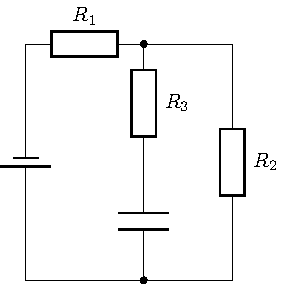
\includegraphics[width = 0.30\textwidth]{Joonis_kondensaator.pdf}
	\end{center}
\end{wrapfigure}


\yl{KONDENSAATOR} Kondensaatorit laetakse kõrvaloleva skeemi järgi alalisvooluallikast pingega $U=\SI{12}{\V}$. Skeemis olevate takistite takistused on vastavalt $R_1=\SI{1}{\kilo\ohm}$, $R_2=\SI{2}{\kilo\ohm}$ ning $R_3=\SI{3}{\kilo\ohm}$. Leida maksimaalne pinge, milleni saame kondensaatori niimoodi laadida. \punktid{8}

\vspace{10pt}
\yl{LENNURADA} Lennuk vajab õhkutõusmiseks vajaliku üleslükkejõu saavutamiseks merepinna kõrgusel vähemalt $L=\SI{2}{km}$ pikkust hoorada. Kui pikka hoorada vajaks sama lennuk maailma kõrgeimal tsiviillennuväljal, mis asub merepinnast $\SI{4}{km}$ kõrgusel? Õhu tihedus merepinnal $\rho_1 = \SI{1,23}{kg/m^3}$ ning $\SI{4}{km}$ kõrgusel $\rho_2 = \SI{0,82 }{kg/m^3}$. Lennuki tiibade poolt tekitatav üleslükkejõud on võrdeline õhu tiheduse ning lennuki kiiruse ruuduga. Eeldada, et ilm on mõlemal juhul tuulevaikne ning lennuki kiirendus on kogu hoovõtu jooksul konstantne. \punktid{8}

\yl{GRANAAT} Granaat visatakse algkiirusega $v$ õhku nurga $\alpha$ all. Hetkel $t_1$ plahvatab granaat $N\gg1$ killuks, kusjuures granaadi massikeskme süsteemis eemalduvad killud kiirusega $u$ ühtlase nurkjaotusega. Mis ajahetkel $t_2$ jõuab esimene kild maapinnani ning mis ajahetkel $t_3$ viimane? Raskuskiirendus on $g$. \punktid{12}

\yl{KIIK} Juku kiigub  nii suure hooga, et kiik jõuab haripunktis kiigepostide (kiige pöörlemistelje) kõrguseni. Suure hoo tõttu hakkab Juku muretsema, kas kiige postid ikka vastu peavad.\\
\osa Leida minimaalne ja maksimaalne jõud, mida Juku kiikumisel postidele avaldab.\\
\osa Leida minimaalne ja maksimaalne jõumoment, mida Juku kiikumisel postidele avaldab. Jõumoment arvutada kiigeposti alumise otsa ehk maasse kinnitamise punkti suhtes.
Kiige võll (pöörlemistelg) on kinnitatud kahe horisontaalse posti otsa kõrgusel $H$ maapinnast. Tasakaaluasendis on Juku masskeskme kõrgus maapinnast h. Juku mass on $m$, raskuskiirendus g. Kiige istme mass lugeda tühiseks. Lihtsustatult võib Jukut vaadelda punktmassina, mille kaugus kiige võllist ei muutu. \punktid{12}



\yl{3 DIOODI} Joonisel näidatud skeem sisaldab kahte ühesugust takistit ($r=\SI {1.0}\ohm$) ning kolme valgusdioodi: sinist, rohelist ja punast, mis on tähistatud vastavalt tähtedega $S$, $R$ ja $P$. Dioodide voolutugevuse sõltuvuse pingest võib lugeda lihtsuse mõttes selliseks nagu näidatud kõrvaloleval graafikul: voolutugevus on null, kui dioodile rakendatud päripinge on väiksem avanemispingest $V_a$ ning suvalise nullist erineva pärivoolu korral on dioodi pinge võrdne $V_a$-ga. Avanemispinged on dioodidel järgmised: sinisel $\SI{3.2}V$, rohelisel  $\SI{2.6}V$ ja punasel  $\SI{1.8}V$. Sisendklemmidele $A$ ja $B$ rakendatakse konstantse voolu allikas, mis hoiab klemmi $A$ siseneva ning klemmist $B$ väljuva voolu võrdse $I=\SI{1.0}A$-ga. Millist võimsust tarbivad dioodid (näidata ära iga dioodi võimsus eraldi)? \punktid{12}

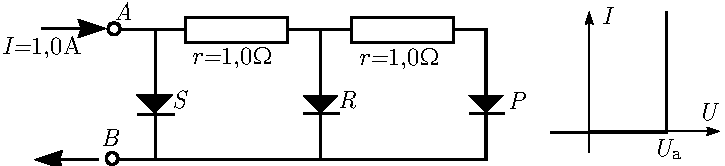
\includegraphics[scale=0.8]{3dioodi}
\end{document}